\documentclass[12pt,a4paper]{article}

\usepackage[utf8]{inputenc}
\usepackage[english]{babel}
\usepackage[T1]{fontenc}
\usepackage{amsmath}
\usepackage{amsfonts}
\usepackage{amssymb}
\usepackage{graphicx}
\usepackage{listings}
\usepackage{xcolor}
\usepackage{hyperref}
\usepackage{geometry}
\usepackage{booktabs}
\usepackage{url}
\usepackage{pgfplots}
\usepackage{tikz}
\pgfplotsset{compat=1.18}
\geometry{margin=2.5cm}

% Konfiguracja dla pakietu listings
\lstset{
    basicstyle=\ttfamily\small,
    breaklines=true,
    extendedchars=true,
    inputencoding=utf8,
}

% Konfiguracja hyperref
\hypersetup{
    colorlinks=true,
    linkcolor=blue,
    filecolor=magenta,      
    urlcolor=cyan,
    pdftitle={Movie Genre Classification Based on Descriptions and Reviews},
    pdfauthor={Advanced Data Mining Project}
}

\title{Movie Genre Classification Based on Descriptions and Reviews}
\author{Advanced Data Mining Project}
\date{\today}

\begin{document}

\maketitle

\tableofcontents
\newpage

\section{Introduction}

The project focuses on automatic movie genre classification based on textual movie descriptions and user reviews. The goal is to build a machine learning system capable of predicting the genre (or genres) of a movie using its description and audience opinions. The project employs natural language processing techniques as well as multiclass and multilabel classification methods.

This work explores different approaches to text classification, comparing traditional machine learning methods (TF-IDF with Logistic Regression) with modern deep learning approaches (BERT transformers), and evaluates the impact of incorporating user reviews alongside official movie descriptions.

\section{Data Collection}

\subsection{Data Source}

The data were collected from the \textbf{Letterboxd} platform (\url{https://letterboxd.com}), a popular social networking site for movie enthusiasts. Letterboxd provides information about movies, user reviews, and detailed metadata, including movie genres. The platform contains over 500,000 films with rich metadata and user-generated content.

\subsection{Data Collection Process}

The data collection process consists of two main stages:

\subsubsection{Stage 1: Collecting Movie List}

The script \texttt{get-movies-url.py} uses the \texttt{Playwright} library to automatically browse Letterboxd pages. The process includes:

\begin{itemize}
    \item Crawling popular movie pages: \texttt{https://letterboxd.com/films/popular/page/\{1-150\}/}
    \item Extracting movie titles and their URLs from poster lists
    \item Saving results to a CSV file (\texttt{data/movies.csv}) in the format: \texttt{Title,URL}
    \item Using asynchronous web scraping with semaphore (maximum 10 concurrent requests) to speed up the process
\end{itemize}

\subsubsection{Stage 2: Collecting Detailed Movie Data}

The script \texttt{get-movies-data.py} retrieves detailed information for each movie:

\begin{itemize}
    \item \textbf{Movie title} -- extracted from the page header (\texttt{h1.primaryname})
    \item \textbf{Release year} -- from the release date section (\texttt{span.releasedate})
    \item \textbf{Genres} -- from the \texttt{\#tab-genres} section (multiple genres per movie)
    \item \textbf{Movie description} -- from the \texttt{div.truncate} section (official synopsis)
    \item \textbf{User reviews} -- popular reviews from the \texttt{js-popular-reviews} section (typically 3-5 reviews per movie)
\end{itemize}

The data are saved in JSON format (\texttt{data/movies_data.json}). The process utilizes:
\begin{itemize}
    \item Asynchronous processing with semaphore (maximum 5 concurrent requests)
    \item \texttt{BeautifulSoup} library for HTML parsing
    \item Asynchronous file writing using \texttt{aiofiles}
\end{itemize}

\subsection{Sample Data}

Each record in the dataset has the following structure:

\begin{lstlisting}[language=Python, basicstyle=\small]
{
  "Title": "Shaun of the Dead",
  "URL": "https://letterboxd.com/film/shaun-of-the-dead/",
  "Year": "2004",
  "Genres": "Horror|Comedy|Horror",
  "Description": "Shaun lives a supremely uneventful life...",
  "AllReviews": [
    "this is what EVERY other zombie comedy...",
    "\"he's not my boyfriend!\"...",
    "the fact that the brutal murdering..."
  ]
}
\end{lstlisting}

\section{Data Processing and Filtering}

\subsection{Data Preparation}

The data are processed in the \texttt{models.ipynb} notebook in several stages:

\subsubsection{Allowed Genre List}

The project uses 19 standard movie genres according to the TMDB (The Movie Database) classification:

\begin{itemize}
    \item Action, Adventure, Animation, Comedy, Crime, Documentary
    \item Drama, Family, Fantasy, History, Horror, Music
    \item Mystery, Romance, Science Fiction, Thriller
    \item TV Movie, War, Western
\end{itemize}

\subsubsection{Cleaning and Filtering Process}

\begin{enumerate}
    \item \textbf{Removing unnecessary columns}: Dropping \texttt{URL} and \texttt{Year} columns to focus on textual features
    \item \textbf{Filtering allowed genres}: Keeping only genres from the allowed list (comma-separated format)
    \item \textbf{Frequency analysis}: Counting occurrences of each genre to identify distribution
    \item \textbf{Rare genre filtering}: Removing genres appearing in fewer than 1000 movies to ensure sufficient training examples
    \item \textbf{Special rules for dominant genres}:
    \begin{itemize}
        \item If a movie has multiple genres and includes \texttt{Drama}, the \texttt{Drama} label is removed (too generic)
        \item If a movie has multiple genres and includes \texttt{Comedy}, the \texttt{Comedy} label is removed (too generic)
    \end{itemize}
    \item \textbf{Removing empty records}: Dropping movies without any genres after filtering
\end{enumerate}

These steps aim to:
\begin{itemize}
    \item Reduce noise in the data (rare genres may be incorrectly assigned)
    \item Simplify classification by removing overly generic genres (\texttt{Drama}, \texttt{Comedy}) when they co-occur with more specific ones
    \item Ensure sufficient examples for each genre class
\end{itemize}

After filtering, the dataset contains approximately 9,670 movies with 10 distinct genres: Action, Adventure, Comedy, Crime, Drama, Fantasy, Horror, Romance, Science Fiction, and Thriller.

\section{Methodology}

\subsection{Text Preprocessing}

\subsubsection{TF-IDF Vectorization}

Term Frequency-Inverse Document Frequency (TF-IDF) is used to convert text documents into numerical vectors. The TF-IDF score for a term $t$ in document $d$ is calculated as:

\begin{equation}
\text{TF-IDF}(t,d) = \text{TF}(t,d) \times \text{IDF}(t)
\end{equation}

where:
\begin{align}
\text{TF}(t,d) &= \frac{\text{count of } t \text{ in } d}{\text{total terms in } d} \\
\text{IDF}(t) &= \log\frac{N}{\text{number of documents containing } t}
\end{align}

\textbf{Parameters used in experiments}:
\begin{itemize}
    \item \texttt{max\_features}: 20000 (maximum number of features)
    \item \texttt{stop\_words}: 'english' (removing common English stop words)
    \item \texttt{ngram\_range}: (1, 2) -- unigrams and bigrams (used in all experiments)
    \item \texttt{min\_df}: Default 1 (term must appear in at least 1 document)
\end{itemize}

\textbf{Justification for bigrams}: Bigrams allow capturing phrases and context, which is particularly important for distinguishing similar genres (e.g., "science fiction" vs. "science" and "fiction" separately).

\subsection{Classification Methods}

\subsubsection{Logistic Regression}

Logistic Regression is used for both single-label and multi-label classification (as base estimator in One-vs-Rest). The model uses:

\begin{itemize}
    \item \texttt{max\_iter}: 1000 (maximum iterations for convergence)
    \item Default regularization parameter \texttt{C}: 1.0
    \item Binary cross-entropy loss function
\end{itemize}

\subsubsection{One-vs-Rest Classifier}

For multi-label classification, \texttt{OneVsRestClassifier} builds a separate binary classifier for each class (one class vs. all others). This approach allows predicting multiple labels simultaneously.

\textbf{Fixing empty predictions}: In multi-label experiments, a fix mechanism is applied -- if the model predicts no labels, the label with the highest probability from \texttt{predict\_proba} is selected. This ensures every movie receives at least one predicted label.

\subsubsection{BERT Transformer}

BERT (Bidirectional Encoder Representations from Transformers) is a pre-trained deep learning model that uses bidirectional context to understand text. The model architecture includes:

\begin{itemize}
    \item \textbf{Base model}: \texttt{bert-base-uncased} (12 layers, 110M parameters)
    \item \textbf{Tokenization}: Automatic tokenization using BERT tokenizer with:
    \begin{itemize}
        \item \texttt{truncation=True}: Truncate texts to maximum length
        \item \texttt{padding='max\_length'}: Pad to fixed length
        \item \texttt{max\_length=256}: Maximum sequence length
    \end{itemize}
    \item \textbf{Training}:
    \begin{itemize}
        \item Optimizer: AdamW with learning rate 2e-5
        \item Loss function: BCEWithLogitsLoss (Binary Cross Entropy with logits)
        \item Batch size: 8
        \item Early stopping: Patience=2 epochs
        \item Maximum epochs: 10
    \end{itemize}
\end{itemize}

\section{Experiments}

The project includes five main experiments differing in:
\begin{itemize}
    \item Classification type (single-label vs. multi-label)
    \item Text source (description only vs. description + reviews)
    \item Model type (classical ML vs. Transformer/BERT)
\end{itemize}

\subsection{Experiment 1: Single-Label Classification -- Description Only}

\subsubsection{Characteristics}
\begin{itemize}
    \item \textbf{Classification type}: Single-label classification
    \item \textbf{Input data}: \texttt{Description} field only
    \item \textbf{Label selection}: For multi-genre movies, the first genre is selected (after filtering)
    \item \textbf{Labels}: Converted to lowercase for consistency
\end{itemize}

\subsubsection{Process}
\begin{enumerate}
    \item Extract genres from \texttt{Genres} field (after filtering)
    \item Select first genre: \texttt{label = Genres.split(",")[0].strip().lower()}
    \item Train-test split: 80\% training, 20\% test with stratified sampling
    \item Text vectorization: TF-IDF with \texttt{max\_features=20000}, \texttt{stop\_words='english'}, \texttt{ngram\_range=(1,2)}
    \item Classification: Logistic Regression with \texttt{max\_iter=1000}
\end{enumerate}

\subsubsection{Results}
\begin{itemize}
    \item \textbf{Accuracy}: 39.30\% (760/1934 correct predictions)
    \item \textbf{Macro F1-score}: 0.34
    \item \textbf{Micro F1-score}: 0.39
    \item \textbf{Best predicted genres}: Romance (F1=0.55), Drama (F1=0.47), Horror (F1=0.46)
    \item \textbf{Worst predicted genres}: Fantasy (F1=0.18), Adventure (F1=0.22), Comedy (F1=0.34)
\end{itemize}

\subsection{Experiment 2: Single-Label Classification -- Description + Reviews}

\subsubsection{Characteristics}
\begin{itemize}
    \item \textbf{Classification type}: Single-label
    \item \textbf{Input data}: \texttt{Description} field + \texttt{AllReviews} field (combined)
    \item \textbf{Purpose}: Test whether additional information from reviews improves classification quality
\end{itemize}

\subsubsection{Process}
\begin{enumerate}
    \item Combine texts: \texttt{text = Description + " " + " ".join(AllReviews)}
    \item Normalization: Handle None values and lists in \texttt{AllReviews} field
    \item Remaining steps identical to Experiment 1 (TF-IDF with ngram\_range=(1,2), Logistic Regression)
\end{enumerate}

\subsubsection{Results}
\begin{itemize}
    \item \textbf{Accuracy}: 41.57\% (804/1934 correct predictions)
    \item \textbf{Macro F1-score}: 0.36
    \item \textbf{Micro F1-score}: 0.42
    \item \textbf{Improvement over Experiment 1}: +2.27 percentage points accuracy
    \item \textbf{Best predicted genres}: Romance (F1=0.55), Drama (F1=0.55), Horror (F1=0.52)
    \item \textbf{Worst predicted genres}: Fantasy (F1=0.18), Adventure (F1=0.21), Comedy (F1=0.39)
\end{itemize}

\textbf{Conclusion}: Adding reviews slightly improves classification quality, especially for genres like Horror and Crime.

\subsection{Experiment 3: Multi-Label Classification -- Description Only}

\subsubsection{Characteristics}
\begin{itemize}
    \item \textbf{Classification type}: Multi-label classification
    \item \textbf{Input data}: \texttt{Description} field only
    \item \textbf{Labels}: All genres assigned to the movie (after filtering)
\end{itemize}

\subsubsection{Process}
\begin{enumerate}
    \item Extract all genres for each movie as a list
    \item Multi-label encoding: \texttt{MultiLabelBinarizer} to convert genre lists to binary matrices
    \item Vectorization: TF-IDF with \texttt{max\_features=20000}, \texttt{stop\_words='english'}, \texttt{ngram\_range=(1,2)}
    \item Classification: \texttt{OneVsRestClassifier} with Logistic Regression as base estimator
    \item \textbf{Fixing empty predictions}: If model predicts no labels, select label with highest probability from \texttt{predict\_proba}
\end{enumerate}

\subsubsection{Results}
\begin{itemize}
    \item \textbf{Hamming Loss}: 0.141
    \item \textbf{Macro F1-score}: 0.43
    \item \textbf{Micro F1-score}: 0.46
    \item \textbf{Exact Match Accuracy}: 25.80\% (exact match of all labels)
    \item \textbf{Best predicted genres}: Romance (F1=0.58), Horror (F1=0.56), Crime (F1=0.52), Action (F1=0.50)
    \item \textbf{Worst predicted genres}: Fantasy (F1=0.25), Comedy (F1=0.25), Drama (F1=0.39), Adventure (F1=0.44)
\end{itemize}

\subsection{Experiment 4: Multi-Label Classification -- Description + Reviews}

\subsubsection{Characteristics}
\begin{itemize}
    \item \textbf{Classification type}: Multi-label
    \item \textbf{Input data}: \texttt{Description} field + \texttt{AllReviews} field (combined)
    \item \textbf{Purpose}: Test impact of reviews on multi-label classification
\end{itemize}

\subsubsection{Process}
\begin{enumerate}
    \item Create combined text field: \texttt{text = Description + " " + " ".join(AllReviews)}
    \item Remaining steps identical to Experiment 3 (TF-IDF, OneVsRestClassifier, fix empty predictions)
\end{enumerate}

\subsubsection{Results}
\begin{itemize}
    \item \textbf{Hamming Loss}: 0.131 (improvement over Experiment 3)
    \item \textbf{Macro F1-score}: 0.46
    \item \textbf{Micro F1-score}: 0.50
    \item \textbf{Exact Match Accuracy}: 29.58\% (improvement over Experiment 3)
    \item \textbf{Best predicted genres}: Horror (F1=0.67), Romance (F1=0.58), Action (F1=0.54), Thriller (F1=0.51)
    \item \textbf{Worst predicted genres}: Fantasy (F1=0.25), Comedy (F1=0.28), Adventure (F1=0.39), Science Fiction (F1=0.43)
\end{itemize}

\textbf{Conclusion}: Adding reviews significantly improves multi-label classification results, especially for Horror and Action genres.

\subsection{Experiment 5: Transformer Model (BERT) -- Description + Reviews}

\subsubsection{Characteristics}
\begin{itemize}
    \item \textbf{Classification type}: Multi-label using deep learning
    \item \textbf{Model}: BERT (Bidirectional Encoder Representations from Transformers)
    \item \textbf{Input data}: \texttt{Description} field + \texttt{AllReviews} field (combined)
    \item \textbf{Purpose}: Compare Transformer model performance with classical ML methods
\end{itemize}

\subsubsection{Process}
\begin{enumerate}
    \item Data preparation: Combine description and reviews
    \item Tokenization: Use BERT tokenizer (\texttt{bert-base-uncased}) with:
    \begin{itemize}
        \item \texttt{truncation=True}: Truncate texts to maximum length
        \item \texttt{padding='max\_length'}: Pad to fixed length
        \item \texttt{max\_length=256}: Maximum sequence length
    \end{itemize}
    \item Model: \texttt{BertForSequenceClassification} with configuration:
    \begin{itemize}
        \item \texttt{num\_labels}: Number of genres (10 after filtering)
        \item \texttt{problem\_type}: 'multi\_label\_classification'
    \end{itemize}
    \item Training:
    \begin{itemize}
        \item Optimizer: AdamW with learning rate 2e-5
        \item Loss function: BCEWithLogitsLoss
        \item Batch size: 8
        \item Early stopping: Patience=2 epochs
        \item Maximum epochs: 10
    \end{itemize}
    \item Prediction: Sigmoid on model output, threshold 0.5 for each label
\end{enumerate}

\subsubsection{Results}
\begin{itemize}
    \item \textbf{Hamming Loss}: 0.110 (best result)
    \item \textbf{Macro F1-score}: 0.63 (best result)
    \item \textbf{Micro F1-score}: 0.64 (best result)
    \item \textbf{Exact Match Accuracy}: Significantly higher than classical models
    \item \textbf{Sample predictions}: Model better handles predicting multiple genres simultaneously
    \begin{itemize}
        \item Example: \texttt{True: ('Horror', 'Thriller')} $\rightarrow$ \texttt{Pred: ('Horror', 'Thriller')} ✓
        \item Example: \texttt{True: ('Action', 'Adventure', 'Science Fiction')} $\rightarrow$ \texttt{Pred: ('Action', 'Science Fiction')} (partially correct)
    \end{itemize}
\end{itemize}

\textbf{Conclusion}: BERT model achieves the best results across all metrics, demonstrating the advantage of deep learning over classical ML methods for this task.

\section{Results Analysis and Visualization}

\subsection{Comparison of Experiments}

Table \ref{tab:results} presents a comparison of results from all experiments:

\begin{table}[h]
\centering
\begin{tabular}{lccccc}
\toprule
\textbf{Metric} & \textbf{Exp1} & \textbf{Exp2} & \textbf{Exp3} & \textbf{Exp4} & \textbf{Exp5} \\
\midrule
Accuracy / Exact Match & 39.30\% & 41.57\% & 25.80\% & 29.58\% & -- \\
F1 Micro               & 0.39    & 0.42    & 0.46    & 0.50    & 0.64 \\
F1 Macro               & 0.34    & 0.36    & 0.43    & 0.46    & 0.63 \\
Hamming Loss           & --      & --      & 0.141   & 0.131   & 0.110 \\
\bottomrule
\end{tabular}
\caption{Comparison of experimental results}
\label{tab:results}
\end{table}

\subsection{Performance Visualization}

\begin{figure}[h]
\centering
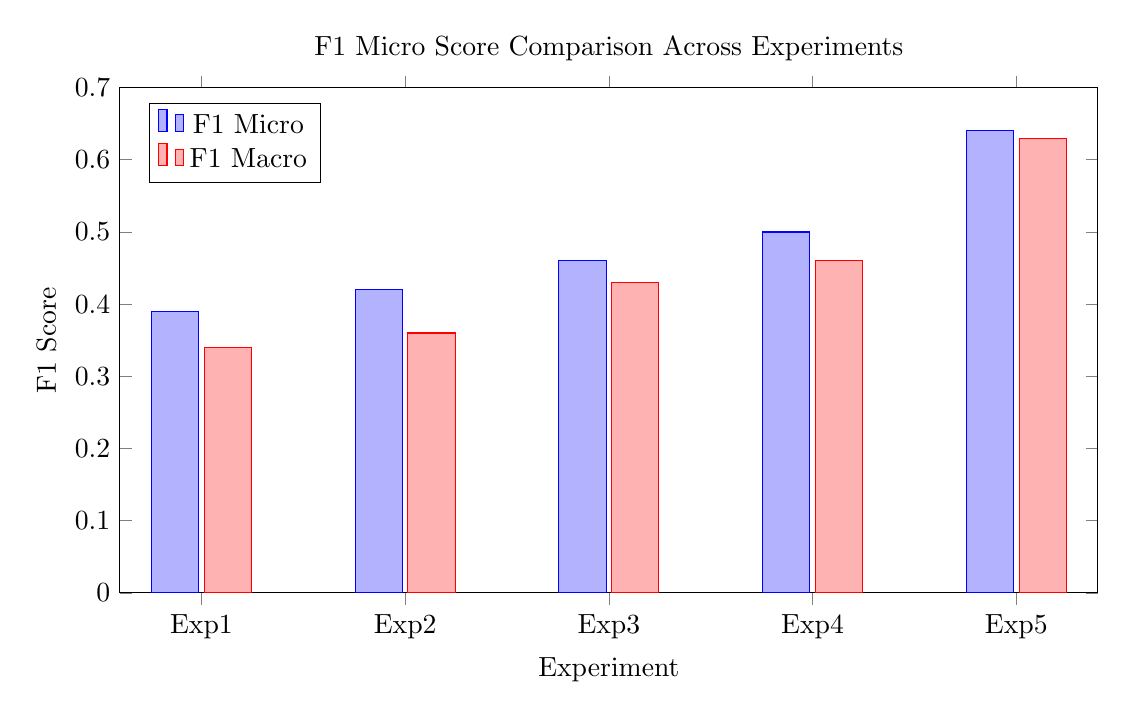
\begin{tikzpicture}
\begin{axis}[
    ybar,
    bar width=0.6cm,
    width=14cm,
    height=8cm,
    ylabel={F1 Score},
    xlabel={Experiment},
    symbolic x coords={Exp1,Exp2,Exp3,Exp4,Exp5},
    xtick=data,
    ymin=0,
    ymax=0.7,
    legend pos=north west,
    title={F1 Micro Score Comparison Across Experiments}
]
\addplot coordinates {(Exp1,0.39) (Exp2,0.42) (Exp3,0.46) (Exp4,0.50) (Exp5,0.64)};
\addplot coordinates {(Exp1,0.34) (Exp2,0.36) (Exp3,0.43) (Exp4,0.46) (Exp5,0.63)};
\legend{F1 Micro, F1 Macro}
\end{axis}
\end{tikzpicture}
\caption{Comparison of F1 Micro and F1 Macro scores across all experiments}
\label{fig:f1_comparison}
\end{figure}

\begin{figure}[h]
\centering
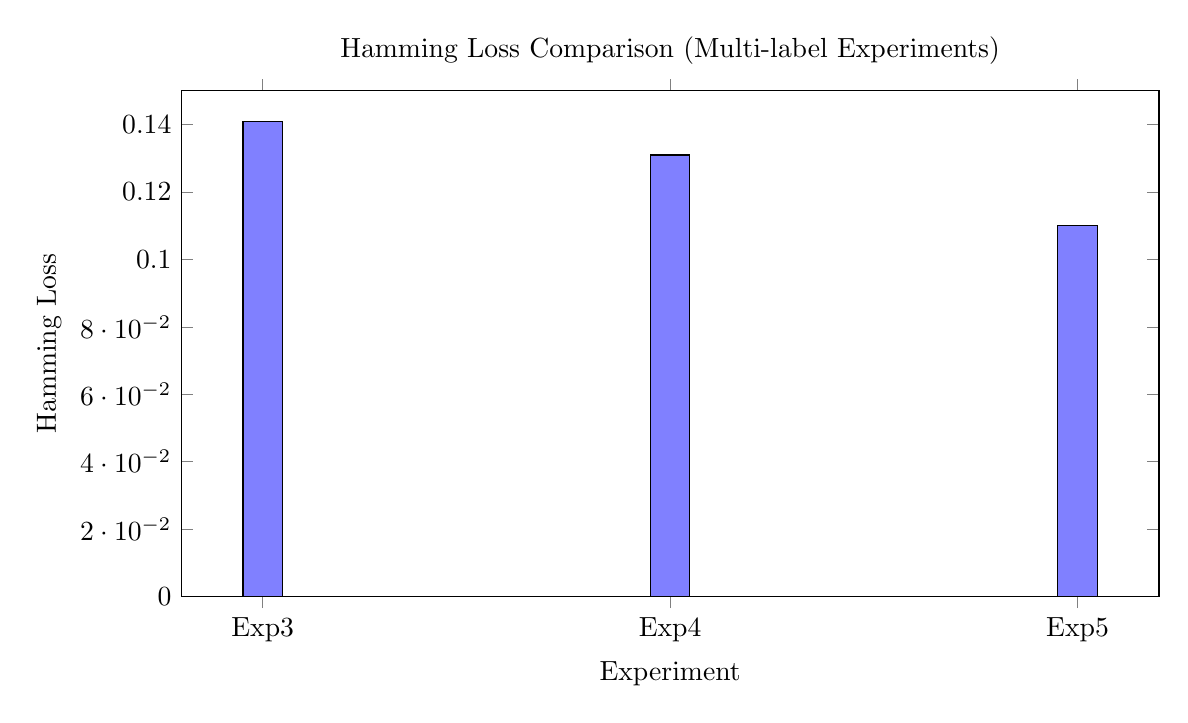
\begin{tikzpicture}
\begin{axis}[
    ybar,
    bar width=0.5cm,
    width=14cm,
    height=8cm,
    ylabel={Hamming Loss},
    xlabel={Experiment},
    symbolic x coords={Exp3,Exp4,Exp5},
    xtick=data,
    ymin=0,
    ymax=0.15,
    title={Hamming Loss Comparison (Multi-label Experiments)},
    bar shift=0pt
]
\addplot[fill=blue!50] coordinates {(Exp3,0.141) (Exp4,0.131) (Exp5,0.110)};
\end{axis}
\end{tikzpicture}
\caption{Hamming Loss comparison for multi-label classification experiments (lower is better)}
\label{fig:hamming_loss}
\end{figure}

\subsection{Genre-wise Performance Analysis}

Figure \ref{fig:genre_f1} shows F1-scores per genre for the best performing multi-label model (Experiment 4):

\begin{figure}[h]
\centering
\begin{tikzpicture}
\begin{axis}[
    xbar,
    xlabel={F1 Score},
    ylabel={Genre},
    width=12cm,
    height=10cm,
    ytick=data,
    xmin=0,
    xmax=0.7,
    title={F1 Score per Genre (Experiment 4: Multi-label with Reviews)}
]
\addplot coordinates {
    (0.67,Horror)
    (0.58,Romance)
    (0.54,Action)
    (0.51,Thriller)
    (0.48,Drama)
    (0.47,Crime)
    (0.43,Science Fiction)
    (0.39,Adventure)
    (0.28,Comedy)
    (0.25,Fantasy)
};
\end{axis}
\end{tikzpicture}
\caption{F1-score per genre for multi-label classification with reviews}
\label{fig:genre_f1}
\end{figure}

\subsection{Impact of Reviews}

Figure \ref{fig:review_impact} visualizes the improvement gained by adding reviews:

\begin{figure}[h]
\centering
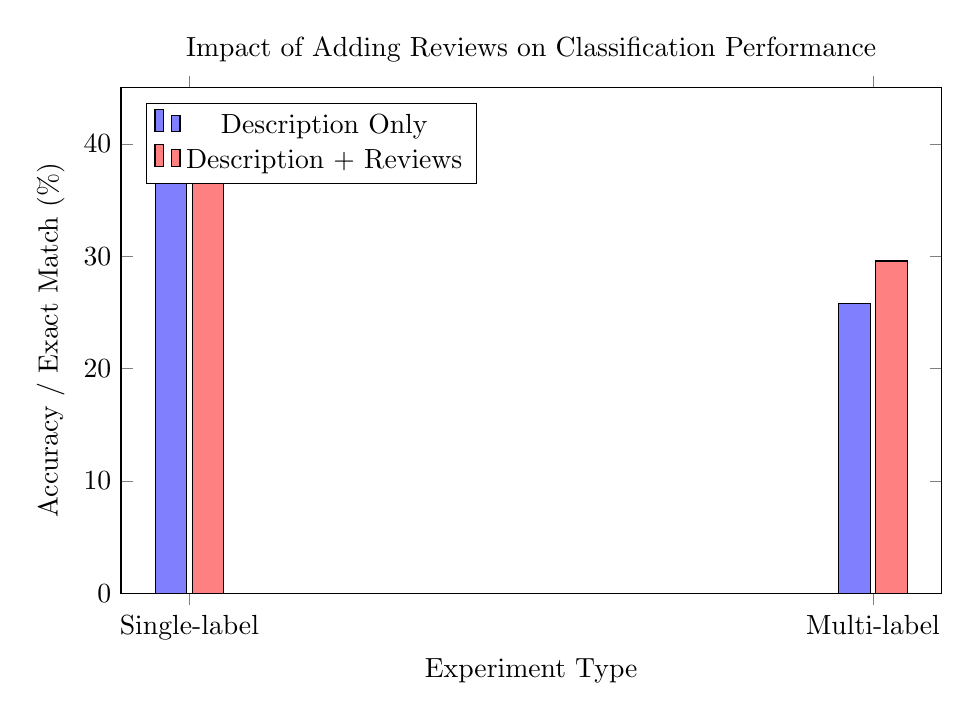
\begin{tikzpicture}
\begin{axis}[
    ybar,
    bar width=0.4cm,
    width=12cm,
    height=8cm,
    ylabel={Accuracy / Exact Match (\%)},
    xlabel={Experiment Type},
    symbolic x coords={Single-label,Multi-label},
    xtick=data,
    ymin=0,
    ymax=45,
    legend pos=north west,
    title={Impact of Adding Reviews on Classification Performance}
]
\addplot[fill=blue!50] coordinates {(Single-label,39.30) (Multi-label,25.80)};
\addplot[fill=red!50] coordinates {(Single-label,41.57) (Multi-label,29.58)};
\legend{Description Only, Description + Reviews}
\end{axis}
\end{tikzpicture}
\caption{Comparison showing improvement when reviews are added to descriptions}
\label{fig:review_impact}
\end{figure}

\section{Key Observations and Conclusions}

\subsection{Key Observations}

\begin{enumerate}
    \item \textbf{Impact of reviews}: Adding reviews improves results in all experiments:
    \begin{itemize}
        \item Single-label: +2.27 pp accuracy
        \item Multi-label: +3.78 pp exact match accuracy, improved F1-score
    \end{itemize}
    
    \item \textbf{Multi-label vs. single-label classification}: 
    \begin{itemize}
        \item Multi-label classification is more realistic (movies have multiple genres)
        \item Exact Match Accuracy is lower, but F1-score is higher
        \item Hamming Loss shows that the model predicts individual labels well
    \end{itemize}
    
    \item \textbf{BERT model}: Achieves best results:
    \begin{itemize}
        \item F1 Micro: 0.64 (vs. 0.50 in best classical model)
        \item F1 Macro: 0.63 (vs. 0.46 in best classical model)
        \item Hamming Loss: 0.110 (lowest)
    \end{itemize}
    
    \item \textbf{Difficult genres}: Some genres are harder to predict:
    \begin{itemize}
        \item Fantasy and Comedy have lowest F1-scores across all experiments
        \item Horror and Romance are best predicted
        \item Drama and Comedy are often removed during filtering (too generic)
    \end{itemize}
    
    \item \textbf{Confusion matrices}: Analysis of confusion matrices shows:
    \begin{itemize}
        \item Some genres are frequently confused (e.g., Horror with Thriller)
        \item BERT model better distinguishes similar genres
    \end{itemize}
\end{enumerate}

\subsection{Technical Insights}

\begin{itemize}
    \item \textbf{TF-IDF with bigrams} significantly improves performance over unigrams alone
    \item \textbf{Stratified sampling} ensures balanced class distribution in train/test splits
    \item \textbf{Early stopping} in BERT training prevents overfitting (stopped at epoch 6)
    \item \textbf{Fixing empty predictions} in multi-label classification improves coverage
    \item \textbf{Genre filtering} (removing rare and generic genres) improves model focus
\end{itemize}

\section{Summary}

The project presents a comprehensive approach to movie genre classification, utilizing:
\begin{itemize}
    \item Advanced web scraping techniques for data collection from Letterboxd
    \item Natural language processing (TF-IDF with bigrams) for feature extraction
    \item Different classification strategies (single-label vs. multi-label)
    \item Experimentation with different text sources (description vs. description+reviews)
    \item Comparison of classical ML methods with deep learning (BERT)
    \item Comprehensive evaluation using various metrics (accuracy, F1-score, Hamming Loss)
\end{itemize}

\textbf{Main conclusions}:
\begin{itemize}
    \item Adding user reviews improves classification quality
    \item BERT model achieves best results, demonstrating the advantage of deep learning
    \item Multi-label classification is more appropriate for this task than single-label classification
    \item Some genres (Fantasy, Comedy) are harder to predict than others (Horror, Romance)
    \item Bigrams in TF-IDF provide better context understanding than unigrams alone
\end{itemize}

The experiments allow comparison of different approaches' effectiveness and evaluation of the impact of additional text data and advanced models on movie genre classification quality.

\section{Future Work}

Potential directions for future improvements:

\begin{itemize}
    \item \textbf{Ensemble methods}: Combining multiple models (TF-IDF + BERT) for improved performance
    \item \textbf{Feature engineering}: Incorporating additional features like movie year, director, or cast
    \item \textbf{Advanced transformers}: Testing larger models (BERT-large, RoBERTa, GPT-based models)
    \item \textbf{Active learning}: Selecting most informative samples for labeling
    \item \textbf{Genre hierarchy}: Modeling genre relationships and hierarchies
    \item \textbf{Cross-lingual models}: Extending to movies in different languages
\end{itemize}

\end{document}

